\documentclass[tikz, border=1mm]{standalone}
\begin{document}
    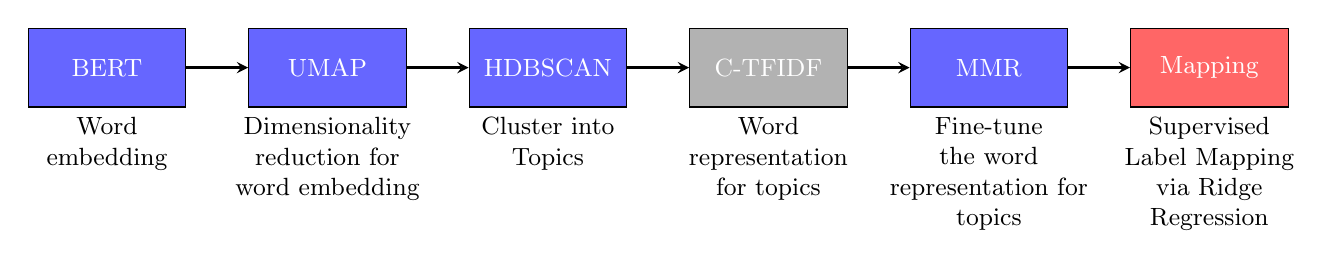
\begin{tikzpicture}[node distance=2.8cm, every node/.style={font=\small}]
    % Styles
    \tikzstyle{method} = [rectangle, minimum width=2cm, minimum height=1cm, text centered, draw=black, fill=blue!60, text=white]
    \tikzstyle{arrow} = [thick,->,>=stealth]
    \tikzstyle{caption} = [below, align=center]

    % Nodes
    \node (bert)   [method] {BERT};
    \node (umap)   [method, right of=bert] {UMAP};
    \node (hdbscan) [method, right of=umap] {HDBSCAN};
    \node (ctfidf) [method, right of=hdbscan, fill=gray!60] {C-TFIDF};
    \node (mmr)    [method, right of=ctfidf] {MMR};
    \node (mapping)    [method, right of=mmr, fill=red!60] {Mapping};

    % Arrows
    \draw [arrow] (bert) -- (umap);
    \draw [arrow] (umap) -- (hdbscan);
    \draw [arrow] (hdbscan) -- (ctfidf);
    \draw [arrow] (ctfidf) -- (mmr);
    \draw [arrow] (mmr) -- (mapping);

    % Captions
    \node [caption] at (bert.south)   {Word\\embedding};
    \node [caption] at (umap.south)   {Dimensionality\\reduction for\\word embedding};
    \node [caption] at (hdbscan.south){Cluster into\\Topics};
    \node [caption] at (ctfidf.south) {Word\\representation\\for topics};
    \node [caption] at (mmr.south)    {Fine-tune\\the word\\representation for\\topics};
    \node [caption] at (mapping.south)    {Supervised\\Label Mapping\\via Ridge\\Regression};
    \end{tikzpicture}
\end{document}